\chapter{Control}\label{ch:control}




\title{Control}

\title{cruise control}

In this chapter we will look more closely at the cruise controller developed for the robot. Cruise control is essential for the robot since it ensures, that it keeps following a straight line and in certain angle respect to the global co-ordinate axis. The motor model used in this chapter is the same one that we examined in the previous one. The before discussed motor model is completely linear, in what case we can apply classical control techniques in order to design the controller.

In the cruise control we want to manipulate the velocity and the angular speed of the robot. In order to do that we must be abel to control each of the wheels angular speed namely $\omega_{r}$ and $\omega_{l}$.

{\color{red} HERE GOES A FIGURE WHAT SHOWS ROBOT IN GLOBAL CO-ORDINATES}

In the following figure you can see the closed loop block diagram for the motor speed control. The plant in this diagram is the same motor model as we looked in the previous chapter.

\begin{figure}[H]

	
	\centering
 	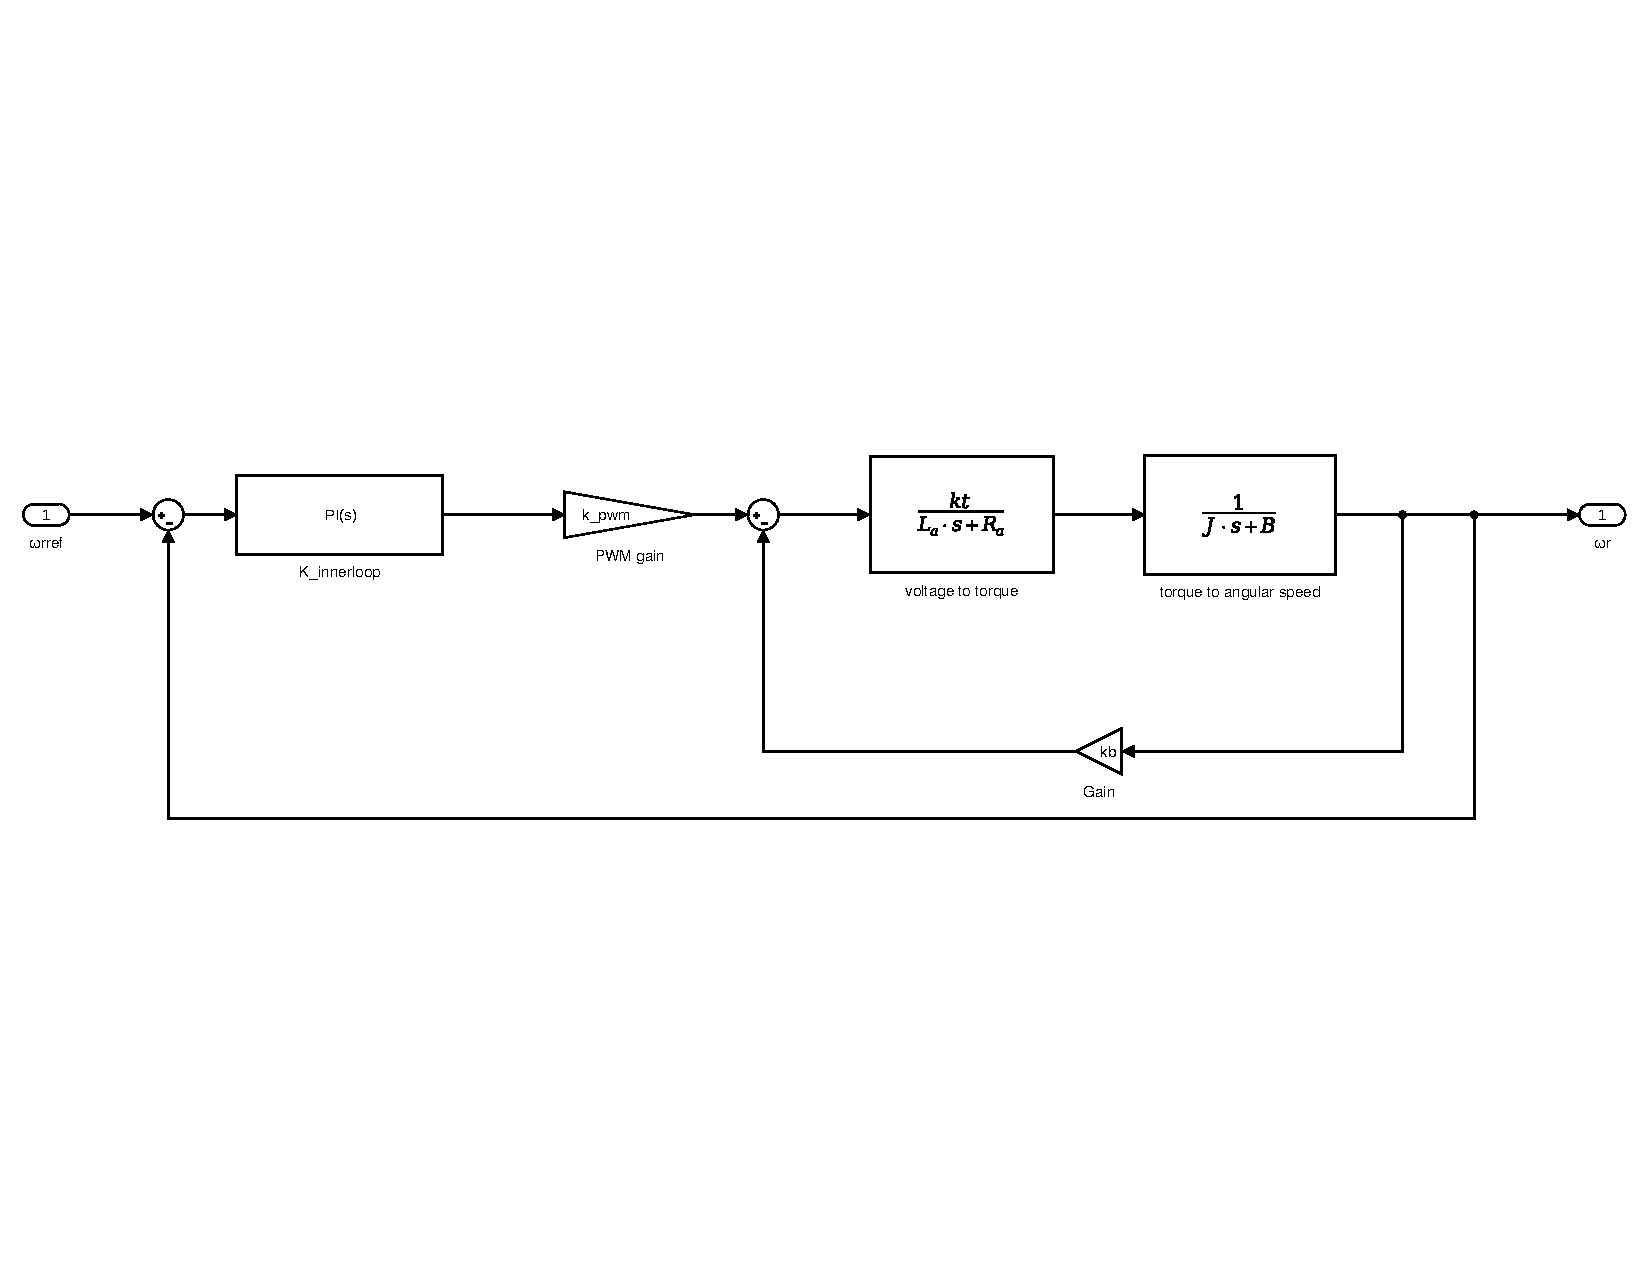
\includegraphics[width=1\textwidth]{figures/motorspeedcontrolclosedloop.pdf}
	
	
	\caption{Motor speed control} 
 	\label{fig:speedcontrol} 
\end{figure}

Now we will look more closely what is in that diagram. First we have the plant model whit what are we already familiar. Next we have the $K_{innerloop}$, what is the PI controller what we have designed to meet our desires. From the diagram we can see that we will have an $P_{innerloop}$ what is the motor model and the PWM term $k_{pwm}$ put together. As a result we get the following equation:

\begin{equation}
P_{innerloop}=\frac{k.k_{pwm}}{k^2+(sL_{a}+R_{a})(sJ+B)}=\frac{3300}{(s+1.02)(s+5000)}
\end{equation}

Next we will look at the $K_{innerloop}$. This is the PI controller what we have developed for the system in order to meet the desired specifications. 

\begin{equation}
K_{innerloop}=\frac{g(s+z)}{s}*[\frac{100}{s+100}]^2
\end{equation} 

Following we can see that the open loop transfer function is given by the following equation:

\begin{equation}
G_{innerloop}=P_{innerloop}*K_{innerloop}
\end{equation}

and the closedloop transfer function we get:

\begin{equation}
H_{innerloop}=\frac{G_{innerloop}}{G_{innerloop}+1}
\end{equation}

For the simulations we used three different values on the g and z. For the first simulation we used z=1 and g=7. In the second simulation we used z=5 and g=5. for the final one we used z=10 and g=6.

The bode plots of the simulation can be seen below.

\begin{figure}
\centering
 	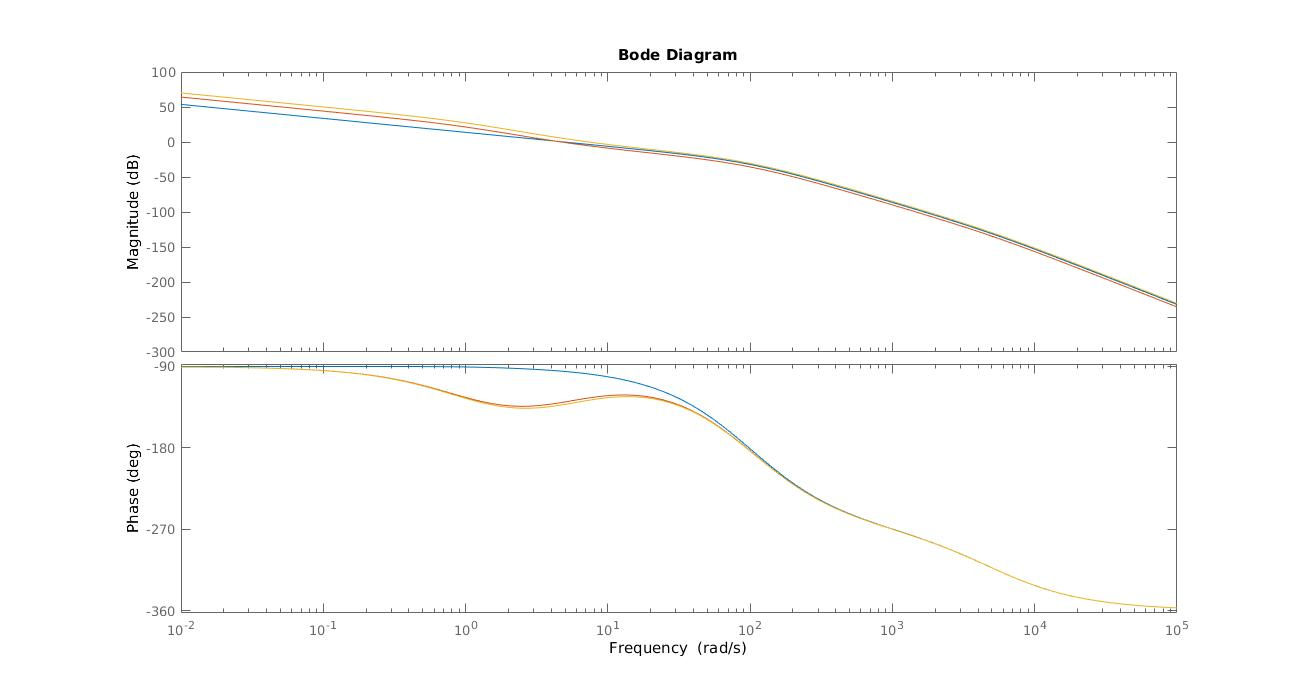
\includegraphics[width=1\textwidth]{figures/Ginnerbode.jpg}
	
	
	\caption{$G_{innerloop}$ bode plot} 
 	\label{fig:ginnerloopbode} 
\end{figure}

\begin{figure}
\centering
 	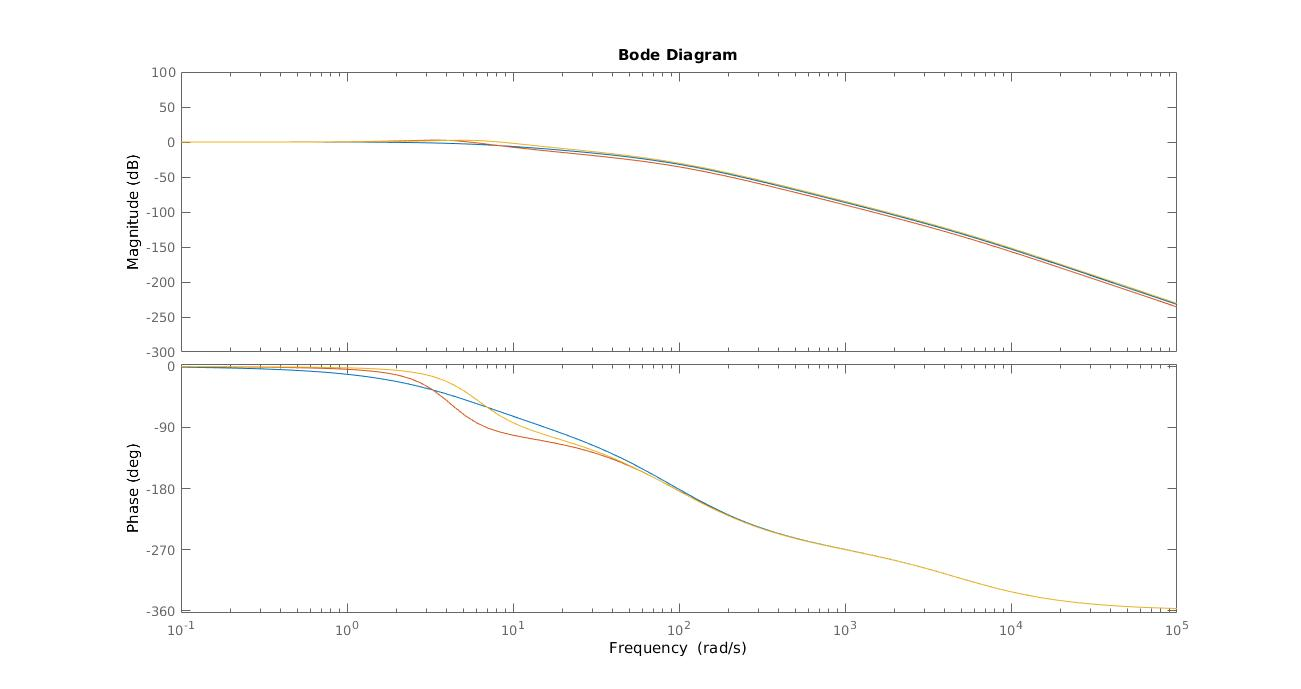
\includegraphics[width=1\textwidth]{figures/Hinnerbode.jpg}
	
	
	\caption{$H_{innerloop}$ bode plot} 
 	\label{fig:hinnerloopbode} 
\end{figure}

From the next figure you can see the step responses of the three different settings on controllers.

\begin{figure}
\centering
 	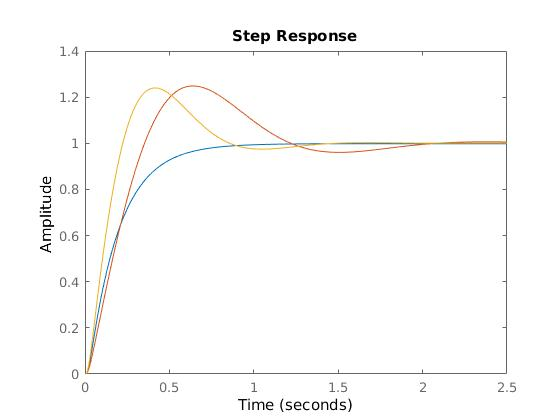
\includegraphics[width=1\textwidth]{figures/stepresponse.jpg}
	
	
	\caption{Step response} 
 	\label{fig:stepresponse} 
\end{figure}

\title{Controlling the $\theta$}

Previously we looked at the control design of the seperate angular velocities. In this section we will be takeing a closer look on the complete architecture of the cruise control. The whole cruise control layout can be seen in figure~\ref{fig:cruisecontrol}.

In order to develop the architecture of the cruise control we first must look how can we obtain $\omega_{rref}$ and $\omega_{lref}$ by manipulating $\omega$ and $v$.

\begin{equation} \label{eq66}
 \begin{pmatrix} 
 \omega_{rref} \\ 
 \omega_{lref} \\
 \end{pmatrix} 
 =
 \begin{pmatrix}  
 \frac{1}{R}   & \frac{L}{2R} \\ 
 \frac{1}{R} & \frac{-L}{2R} \\ 
 \end{pmatrix}
 \begin{pmatrix} 
 v_{ref} \\ 
 \omega_{ref}
 \end{pmatrix} 
 \end{equation} 

\begin{equation} \label{eq67}
M^{-1}
=
\begin{pmatrix}  
 \frac{1}{R}   & \frac{L}{2R} \\ 
 \frac{1}{R} & \frac{-L}{2R} \\ 
 \end{pmatrix} 
\end{equation}

\begin{figure}
\centering
 	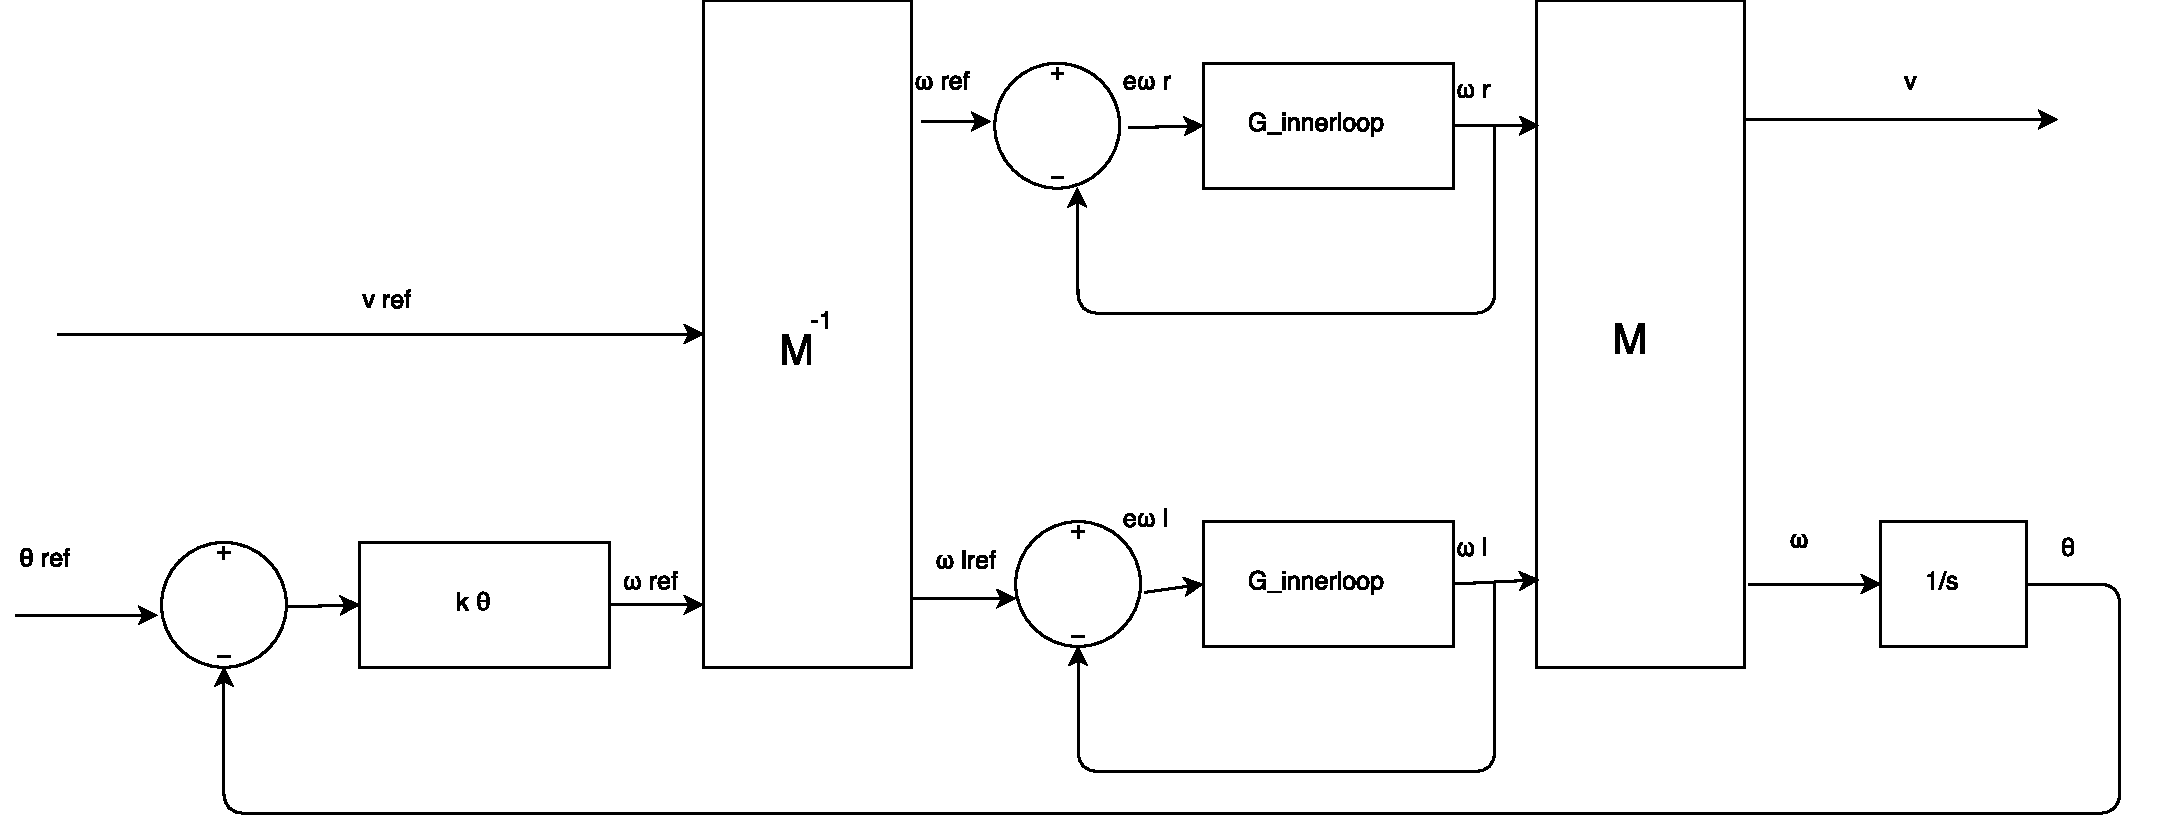
\includegraphics[width=1\textwidth]{figures/cruisecontrol.pdf}
	\caption{Cruise control full architecture} 
 	\label{fig:cruisecontrol} 
\end{figure}

In the equations \ref{eq66} and \ref{eq67} we have $\omega_{rref}$ and $\omega_{lref}$ what are the seperate wheels angular speeds what are commanded by the system. $v_{ref}$ is the linear speed on the robot and $\omega_{ref}$ is the desired angular speed of the whole robot. $R$ is the radius of the wheels and $L$ is the lenght between motorized wheels.

By analyzing the equations we can see that the transfer functions from reference linear speed($v_{ref}$) to the linear speed ($v$). Similarly is the transfer function from $\omega_{ref}$ to $\omega$. This will tell us that the $v_{ref}$ to $v$ and $\omega_{ref}$ to $\omega$ time and frequency responses are the same as are the motor speed responses. Using that knowlage we can now obtain new equations\ref{eq68} and \ref{eq69}

\begin{equation} \label{eq68}
 \begin{pmatrix} 
 v(s) \\ 
 \omega(s) \\
 \end{pmatrix} 
 =
 M^{-1}
 \begin{pmatrix}  
 H_{innerloop}(s)   & 0 \\ 
 0 & H_{innerloop}(s) \\ 
 \end{pmatrix}
 M
 \begin{pmatrix} 
 v_{ref}(s) \\ 
 \omega_{ref}(s)
 \end{pmatrix} 
 \end{equation}

\begin{equation} \label{eq69}
\frac{v(s)}{v_{ref}(s)}
=
\frac{\omega(s)}{\omega_{ref}(s)}
=
H_{innerloop}(s)
\end{equation}

In the equations \ref{eq68} and \ref{eq69} the $v_{ref}$ is the linear velocity command and the $\omega_{ref}$ is the angular speed command for the robot.

Next part of the cruise control is to make the robot follow $\Theta_{red}$ the commanded angle. Examining the figure \ref{fig:cruisecontrol} we can see that the plant for the angle control is given by

\begin{equation} \label{eq70}
P_{\Theta}
=
\frac{H_{innerloop}}{s}
=
\frac{24570}{(s+4995)(s+4.957)s}
\end{equation}

For simpler understanding we will simplify the angle control block diagram what can be seen in the figure \ref{fig:anglecontrol}

\begin{figure} 
\centering
 	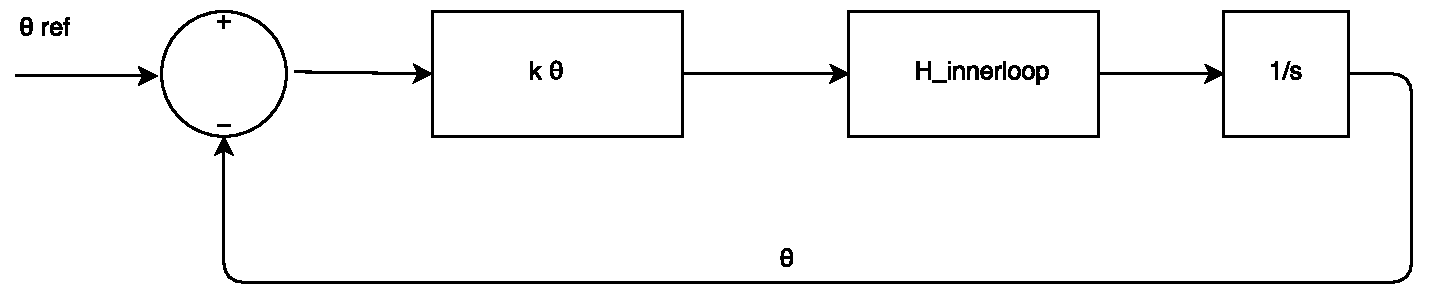
\includegraphics[width=1\textwidth]{figures/cropanglecontrol.pdf}
	
	
	\caption{$\Theta$ control} 
 	\label{fig:anglecontrol} 
\end{figure}

For controlling the $\Theta$ we will use a proportsional controller. The form of the controller $k_{\theta}$ is shown in the equation \ref{eq71}.

\begin{equation} \label{eq71}
k_{\theta}
=
g
\end{equation}

Furthermore we can obtain the transfer function for the open loop loop ($G_{\theta}$) what is given by

\begin{equation} \label{eq72}
G_{\theta}
=
P_{\theta}k_{\theta}
\end{equation}

From here we can get the closed loop loop transfer function, what we will call $H_{\theta}$ shown in the equation \ref{eq73}

\begin{equation} \label{eq73}
H_{\theta}
=
\frac{G_{\theta}}{G_{\theta}+1}
\end{equation}

In the figure \ref{fig:gthetabode} we can see the bode plot of the G_{\theta}. In figure \ref{fig:hthetabode} we have the bode plot of the $H_{\theta}$. And on the figure 

\begin{figure} 
\centering
 	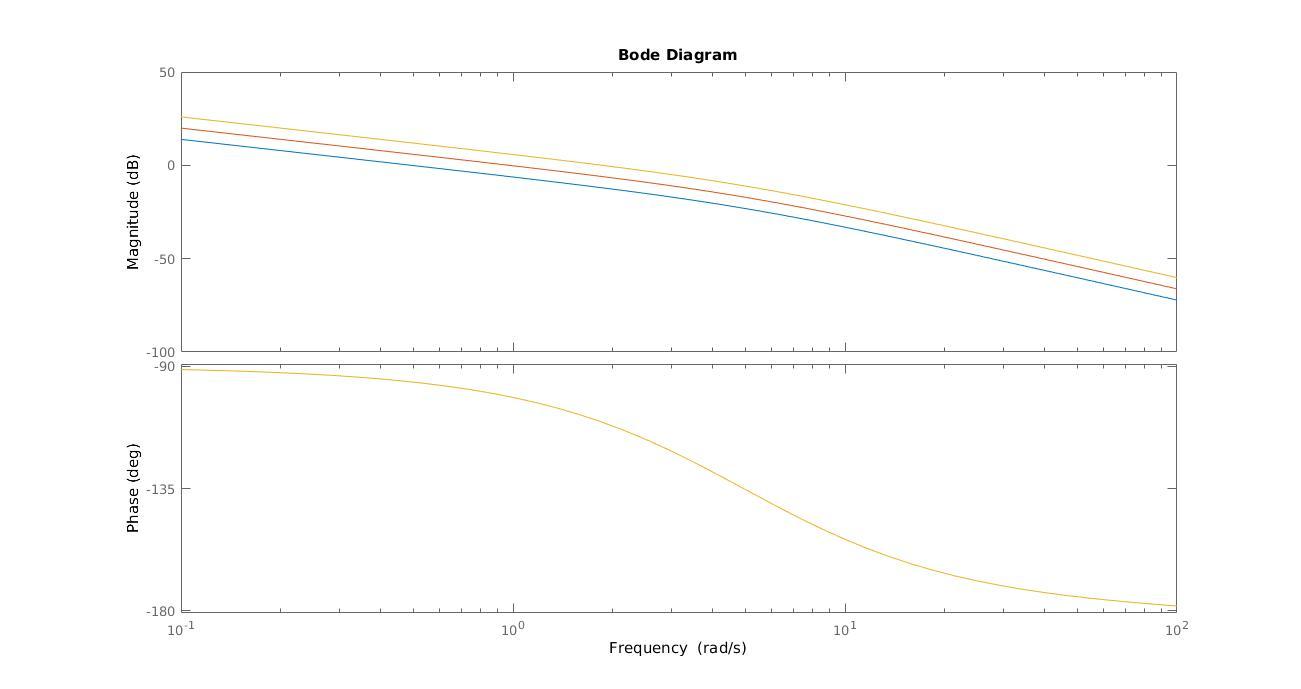
\includegraphics[width=1\textwidth]{figures/G_thetabode.jpg}
	
	
	\caption${G_{\theta}$ bode plot} 
 	\label{fig:gthetabode} 
\end{figure}

\begin{figure} 
\centering
 	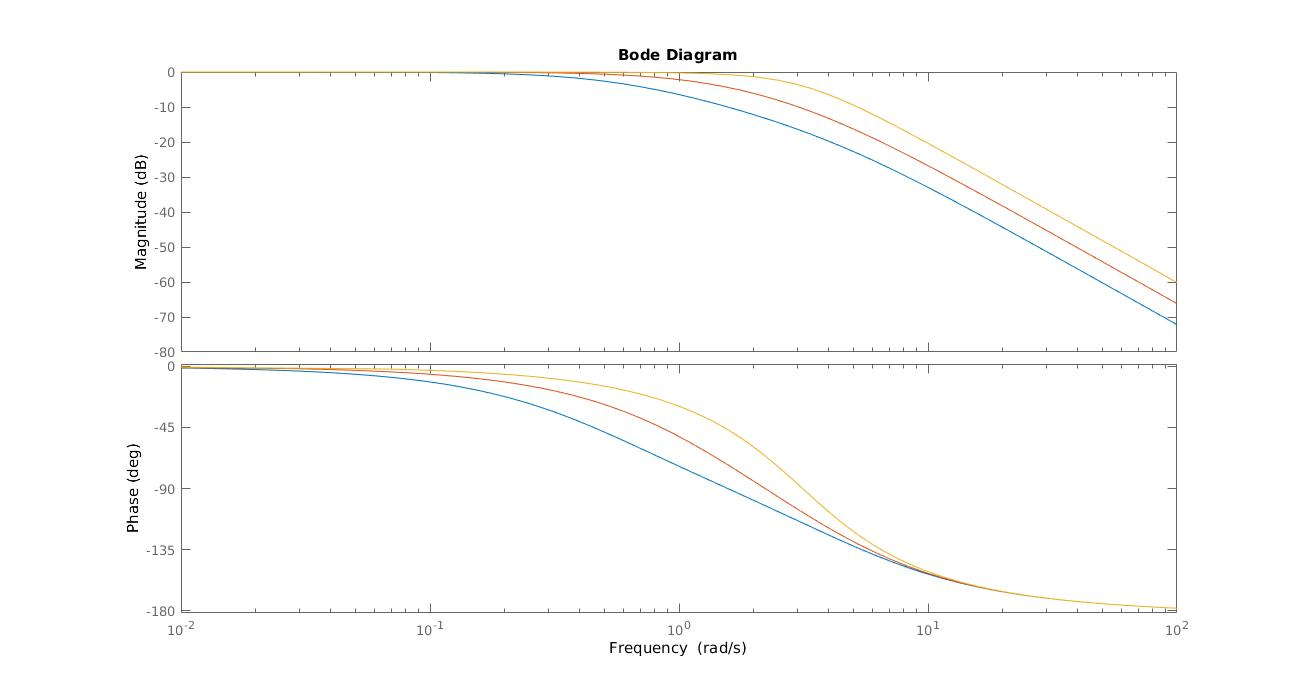
\includegraphics[width=1\textwidth]{figures/Hthetabode.jpg}
	
	
	\caption{$H_{\theta}$ bode plot} 
 	\label{fig:hthetabode} 
\end{figure}

\begin{figure} 
\centering
 	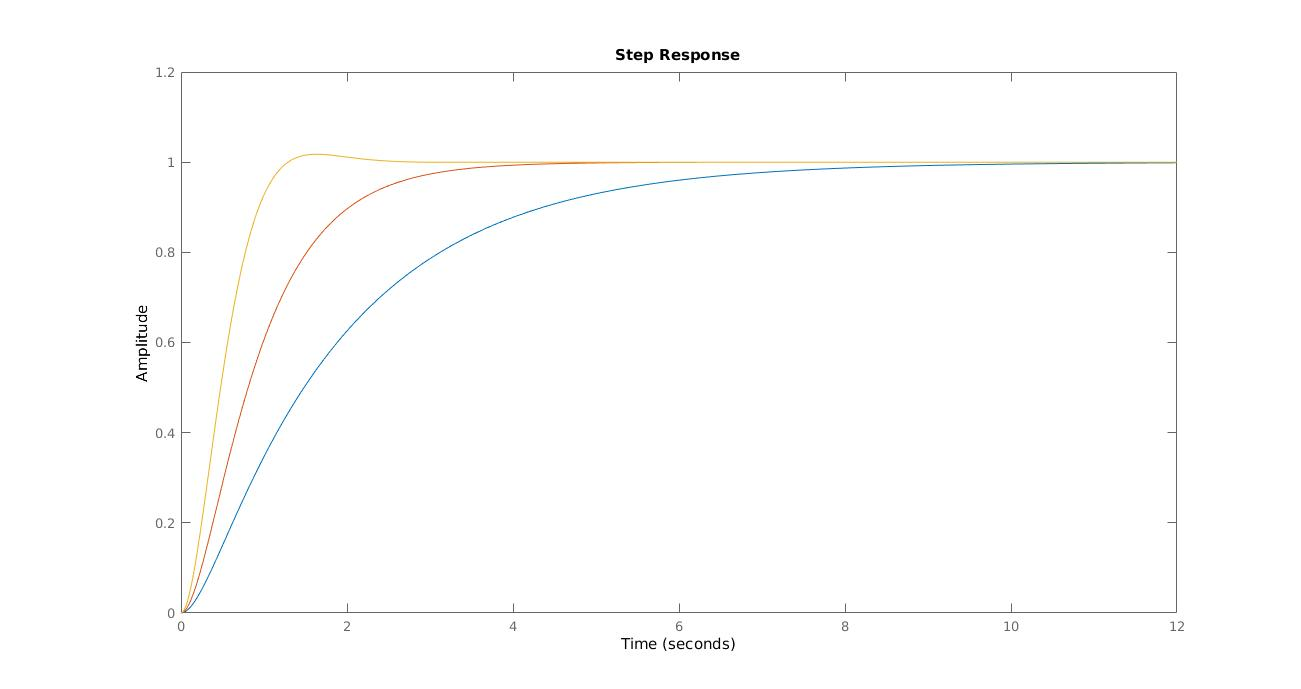
\includegraphics[width=1\textwidth]{figures/thetastep.jpg}
	
	
	\caption{$\Theta$ step response} 
 	\label{fig:thetastep} 
\end{figure}

\title{Kinematic Model Analysis}

A system is said to be controllable if there exists a control law u(.) which can
transfer the state of the system from any initial state x 0 to any final state x f within
a finite amount of time. Otherwise the system is said to be uncontrollable {\color{red} REFERENCE TO sAME BOOK HE HAD}

We will now look more closely the kinematics model and determine if it is controllable or not. The kinematic model is described with the following equations.

\begin{equation} \label{eq74}
\begin{pmatrix} 
 \dot{x} \\ 
 \dot{y} \\
 \dot{\Theta}\\
 \end{pmatrix} 
 =
 \begin{pmatrix}  
 \cos\Theta   & 0 \\ 
 \sin\Theta & 0 \\
 0 & 1\\ 
 \end{pmatrix}
 \begin{pmatrix} 
 v \\ 
 \omega\\
 \end{pmatrix} 
\end{equation}

Since we have the $\sin\Theta$ and $\cos\Theta$ inside the system it is non linear system.

To determine the controllability of the system we must check the sufficient conditions what is given by

\begin{equation} \label{eq75}
rank(h1,h2,[h1,h2])
=
rank
\begin{pmatrix} 
 \cos\Theta & 0 & sin\Theta\\ 
 \sin\Theta & 0 & -\cos\Theta\\
 0 & 1 & 0\\
 \end{pmatrix} 
=
n
=
3
\end{equation}

where

\begin{equation} \label{eq76}
[h1,h2]
=
\frac{\partial h2}{\partial p}h1
-
\frac{\partial h1}{\partial p}h2
\end{equation}

Since we can see that $m$=$n$=3 we can determine that the system is controllable.  This shows us that indeed you can move to any position on the given plain with the robot.

Before we had the kinematic model in the non linear form. Now we will linearize the model about the equilibrium and we obtain the following linearized model of the kinematics.

\begin{equation}
\begin{pmatrix}
\dot{x} \\
\dot{y} \\
\dot{\Theta}
\end{pmatrix}
=
\begin{pmatrix}
1 & 0 \\
0 & 0 \\
0 & 1 \\
\end{pmatrix}
\begin{pmatrix}
v \\
\omega
\end{pmatrix}
\end{equation}

After the linearization we can see that the rank of the controllibility matrix is less then $n$. From that we can only determine that the controllability of the system has been lost after the linearization.

\title{Cartesian Stabilization}

Cartesian stabilisation control is necessary for the robot because it makes sure that the robot goes to the intended point.In the {\color{red}ref to astolfi book} it has been explained the transformation method of the posture stabilization. We will be useing the same method for the cartesian stabilization. 

{\color{red}next subchapter}

First we need to transform the kinematic model \ref{eq74} in the terms of the angular and linear displacements.

\begin{equation}
\dot{s}=v\\
\dot{\Theta}=\omega
\end{equation}

Next we define a new state vector $\rho$

\begin{equation}
\rho
=
\begin{pmatrix}
s\\
\Theta
\end{pmatrix}
\end{equation}

Furthermore we will rewrite the state equations as $\dot{\rho}$.
\begin{equation}
\dot{\rho}=
\begin{pmatrix}
v\\
\omega
\end{pmatrix}
\end{equation}
The transformed system will be used in order to make the robot go towards the goal point. Figure \ref{fig:cartesianstab} shows this system.

\begin{figure} 
\centering
 	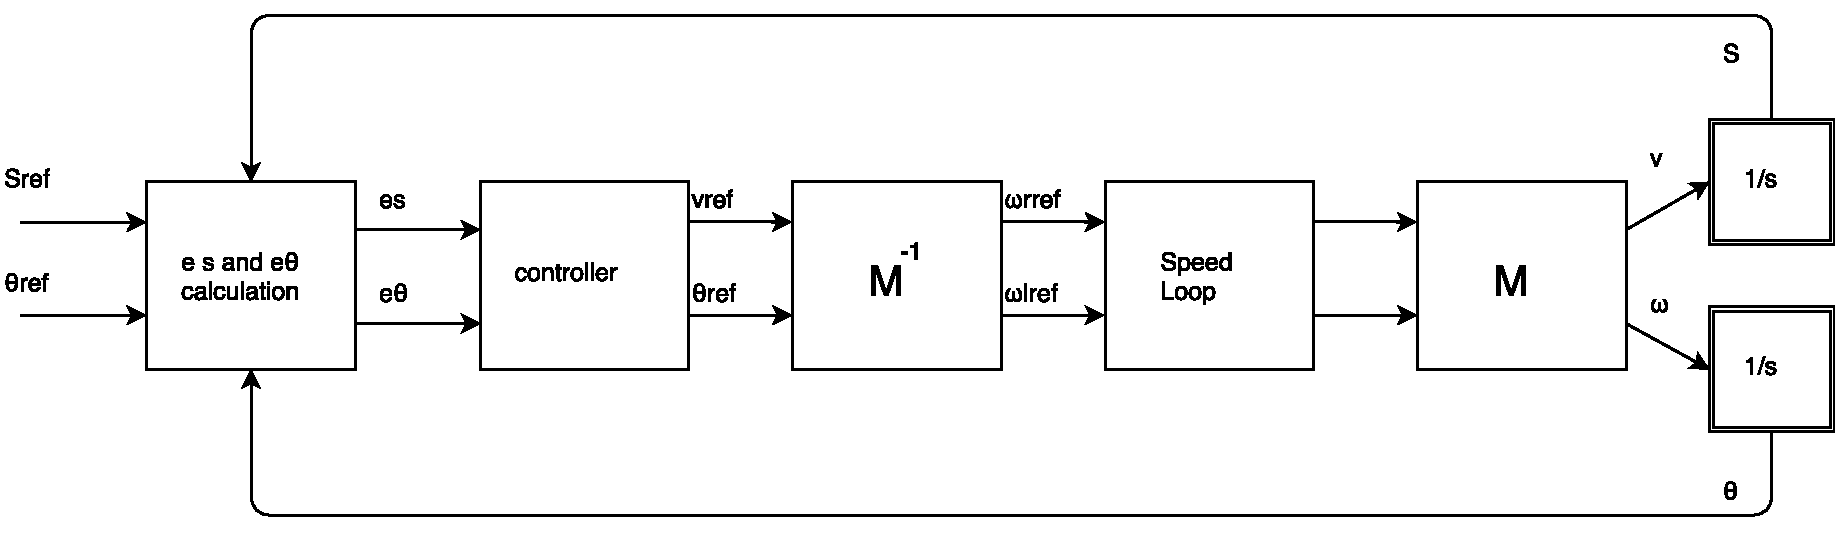
\includegraphics[width=1\textwidth]{figures/cartesianstab.pdf}
	
	
	\caption{Cartesian stabilization} 
 	\label{fig:cartesianstab} 
\end{figure}

As we can see from the figure \ref{fig:cartesianstab} we would neet to get the value of $S_{ref}$. On closer examination we can say that the value of $S_{ref}$ is useless for us and measuring the $S$ is difficult. The problem can be delt with some manipulations as it is explained in{\color{red}Vieira, F.C.; Medeiros, A.A.D.; Alsina P.J.; Araujo A.P. REF THIS}

